	\chapter{Association schemes}\label{association}
	Association schemes arise in group theory, graph theory, design theory, coding theory and more. For example, if $X$ is a finite group with conjugacy classes $\cC[g] = \{hgh^{-1}:h\in X\}$ ($g\in X$), then we find a symmetric association scheme on the vertex set $X$ via merging the relations $R_g\cup R_{g^{-1}}$ where $R_g = \left\{ (a,b) \mid ab^{-1} \in \cC[g]  \right\}$. We find that the group structure is not needed on the point set. In fact, for any point set $X$, the orbits on $X\times X$ of any 
	permutation group $\mathcal{G}$ acting generously transitively also gives an association scheme.
	Some of the most well-studied association schemes are distance-regular graphs, including Moore graphs, distance-transitive graphs, strongly regular graphs, generalized polygons, etc. One studies 
	$q$-ary error-correcting codes of length $n$ as vertex subsets of the Hamming association scheme
	$H(n,q)$ \cite[Sec.~9.2]{Brouwer1989} and $t$-($v,k,\lambda$) designs as vertex subsets of the 
	Johnson association scheme  $J(v,k)$ \cite[Sec.~9.1]{Brouwer1989}.  For an introduction to the 
	extensive literature on the subject, the reader may consult \cite{Delsarte1973,Bannai1984,Brouwer1989,Godsil1993}, 
	the survey \cite{Martin2009}, or the more recent book of  Bailey \cite{Bailey2004} which focuses on 
	connections to the statistical design of experiments.
	\begin{definition}
	Let $X$ be a finite set of vertices. A \textit{symmetric d-class association scheme}\index{association scheme!symmetric} (see \cite{Brouwer1989}) on $X$ is a pair $(X,\mathcal{R})$ where $\mathcal{R} =\left\{R_0,R_1,\dots,R_d\right\}$ is a set of $d+1$ relations on $X$ satisfying the following properties:
	\begin{enumerate}[label=$(\roman*)$]
		\item $R_0$ is the identity relation;
		\item $\left\{R_0,R_1,\dots, R_d\right\}$ forms a partition of $X\times X$;
		\item $(x,y)\in R_i$ implies $(y,x)\in R_i$;
		\item for $0\leq i,j,k\leq d$ there exist constants $p_{i,j}^k$ such that for any $(x,y)\in R_k$, the number of vertices $z$ for which $(x,z)\in R_i$ and $(z,y)\in R_j$ is equal to $p_{i,j}^k$ independent of our original choice of $x$ and $y$.
	\end{enumerate}
	\end{definition}
	The constants $p_{i,j}^k$ are known as the \emph{intersection numbers}\index{parameters!intersection numbers} of our association scheme and we allow ourselves to suppress the comma whenever $i$ and $j$ are given by single digits, thus $p_{5,2}^7$ and $p_{52}^7$ are synonymous throughout this thesis. Properties \emph{(iii)} and \emph{(iv)} together imply that $p_{ij}^k = p_{ji}^k$ for all $i,j,k$; we call such an association scheme \textit{commutative}. There is a broader definition for a \emph{commutative association scheme}\index{association scheme!commutative} where we replace \emph{(iii)} with the requirement that for every $i$, there exists some $i'$ such that $R_{i'} = R_i^T$; that is $(x,y)\in R_i$ if and only if $(y,x)\in R_{i'}$. In this case however, we add the requirement $p_{ij}^k = p_{ji}^k$. Throughout this thesis, all association schemes will be symmetric, though we will add remarks at times when the theorems apply directly to the non-symmetric case as well.
	
	For each $0\leq i\leq d$ we define the (undirected) graph $\Gamma_i = \Gamma(X,R_i)$ on $X$ with $\Gamma_1,\dots,\Gamma_d$ all simple. Note, throughout this thesis we will use the notation $\Gamma(V,E)$ to denote a graph with vertex set $V$ and edge set $E\subset V\times V$. For each $a\in X$ we define the $i^\text{th}$ \emph{neighborhood}\index{relation!neighborhood} of $a$ $R_i(a) = \left\{b\in X\mid (a,b)\in R_i\right\}$; i.e. $R_i(a)$ is the neighborhood of $a$ in the graph $\Gamma_i$. Then for any $a\in X$, the set $X$ is partitioned into the \emph{subconstituents}\index{relation!subconstituents} $\left\{R_i(a)\mid 0\leq i\leq d\right\}$ with respect to $a$.
	\begin{example} The following association scheme is known as the \emph{3-cube}\index{3-cube} with vertex set $X = \left\{0,\dots,7\right\}$ and relations corresponding to the graphs $\Gamma_0,\dots,\Gamma_3$ given below.
		\begin{figure}[H]\begin{center}\scalebox{.7}{$\begin{aligned}
		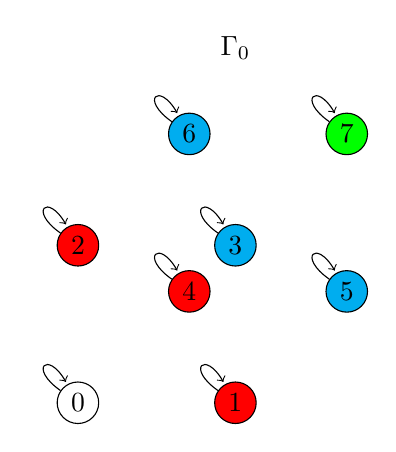
\begin{tikzpicture}[shorten >=1pt,auto,node distance=2cm,
		thin,main node/.style = {circle,draw, inner sep = 0pt, minimum size = 15pt}]
		
		\node[main node,fill=white] (1) {0};
		\node[main node,fill=red] [right of = 1](2) {1};
		\node[main node,fill=red] [above of = 1](3) {2};
		\node[main node,fill=cyan] [right of = 3](4) {3};
		\node[main node,fill=red] [above right of = 1](5) {4};
		\node[main node,fill=cyan] [right of = 5](6) {5};
		\node[main node,fill=cyan] [above of = 5] (7) {6};
		\node[main node,fill=green] [right of = 7](8) {7};
		\node at (2,4.5) (9) {$\Gamma_0$};
		
		\path (1) edge [in=120,out=145,loop] ();
		\path (2) edge [in=120,out=145,loop] ();
		\path (3) edge [in=120,out=145,loop] ();
		\path (4) edge [in=120,out=145,loop] ();
		\path (5) edge [in=120,out=145,loop] ();
		\path (6) edge [in=120,out=145,loop] ();
		\path (7) edge [in=120,out=145,loop] ();
		\path (8) edge [in=120,out=145,loop] ();
		
		\end{tikzpicture}\qquad&\qquad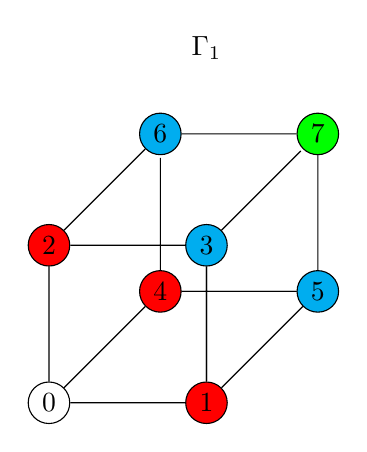
\begin{tikzpicture}[shorten >=1pt,auto,node distance=2cm,
		thin,main node/.style = {circle,draw, inner sep = 0pt, minimum size = 15pt}]
		
		\node[main node,fill=white] (1) {0};
		\node[main node,fill=red] [right of = 1](2) {1};
		\node[main node,fill=red] [above of = 1](3) {2};
		\node[main node,fill=cyan] [right of = 3](4) {3};
		\node[main node,fill=red] [above right of = 1](5) {4};
		\node[main node,fill=cyan] [right of = 5](6) {5};
		\node[main node,fill=cyan] [above of = 5] (7) {6};
		\node[main node,fill=green] [right of = 7](8) {7};
		\node at (2,4.5) (9) {$\Gamma_1$};
		
		\draw[-] (3)--(1)--(2)--(4)--(3)--(7)--(8)--(6)--(5)--(7);
		\draw[-] (1)--(5)--(6)--(2)--(4)--(8);
		\end{tikzpicture}\qquad\qquad
		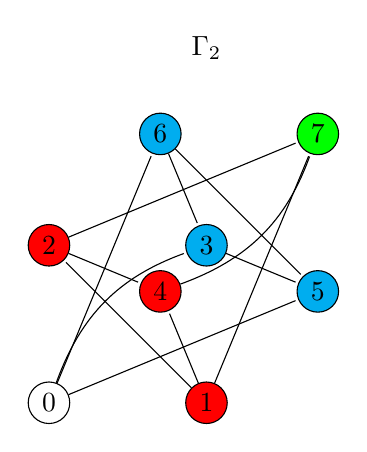
\begin{tikzpicture}[shorten >=1pt,auto,node distance=2cm,
		thin,main node/.style = {circle,draw, inner sep = 0pt, minimum size = 15pt}]
		
		\node[main node,fill=white] (1) {0};
		\node[main node,fill=red] [right of = 1](2) {1};
		\node[main node,fill=red] [above of = 1](3) {2};
		\node[main node,fill=cyan] [right of = 3](4) {3};
		\node[main node,fill=red] [above right of = 1](5) {4};
		\node[main node,fill=cyan] [right of = 5](6) {5};
		\node[main node,fill=cyan] [above of = 5] (7) {6};
		\node[main node,fill=green] [right of = 7](8) {7};
		\node at (2,4.5) (9) {$\Gamma_2$};
		
		\path[-]
		(1)edge [bend left=25] node {} (4)
		edge node {} (6)
		edge node {} (7)
		(2)edge node {} (3)
		edge node {} (5)
		edge node {} (8)
		(3)edge node {} (5)
		edge node {} (8)
		(4) edge node {} (6)
		(7) edge node {} (4)
		edge node {} (6)
		(5) edge [bend right = 25] node {} (8);
		\end{tikzpicture}\qquad&\qquad
		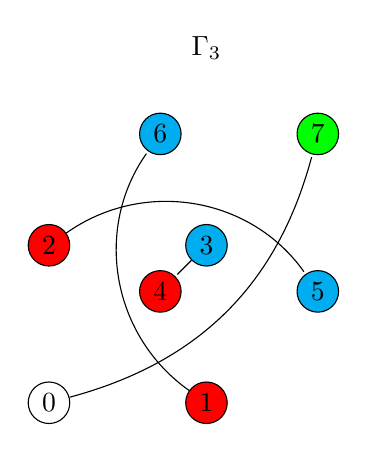
\begin{tikzpicture}[shorten >=1pt,auto,node distance=2cm,
		thin,main node/.style = {circle,draw, inner sep = 0pt, minimum size = 15pt}]
		
		\node[main node,fill=white] (1) {0};
		\node[main node,fill=red] [right of = 1](2) {1};
		\node[main node,fill=red] [above of = 1](3) {2};
		\node[main node,fill=cyan] [right of = 3](4) {3};
		\node[main node,fill=red] [above right of = 1](5) {4};
		\node[main node,fill=cyan] [right of = 5](6) {5};
		\node[main node,fill=cyan] [above of = 5] (7) {6};
		\node[main node,fill=green] [right of = 7](8) {7};
		\node at (2,4.5) (9) {$\Gamma_3$};
		
		\path[-]
		(1) edge [bend right] node {} (8)
		(2) edge [bend left=45] node {} (7)
		(3) edge [bend left=45] node {} (6)
		(4) edge node {} (5);
		\end{tikzpicture}
		\end{aligned}$}\end{center}
		\caption[Graphs of the 3-cube.]{The four graphs of the 3-cube. The four subconstituents of the vertex $0$ are colored white, red, blue, and green respectively.}\label{3cube}
		\end{figure}
		The following matrices give the intersection numbers of this association scheme where the $i^\text{th}$ matrix contains $p^k_{ij}$ with rows indexed by $k$ and columns indexed by $j$:
		\[\left[\begin{array}{cccc}
		1&0&0&0\\
		0&1&0&0\\
		0&0&1&0\\
		0&0&0&1\\
		\end{array}\right],\quad\left[\begin{array}{cccc}
		0&3&0&0\\
		1&0&2&0\\
		0&2&0&1\\
		0&0&3&0\\
		\end{array}\right],\quad\left[\begin{array}{cccc}
		0&0&3&0\\
		0&2&0&1\\
		1&0&2&0\\
		0&3&0&0\\
		\end{array}\right],\quad\left[\begin{array}{cccc}
		0&0&0&1\\
		0&0&1&0\\
		0&1&0&0\\
		1&0&0&0\\
		\end{array}\right].\]
		Since $p^k_{ij} = p^k_{ji}$, many of the columns listed above are redundant, thus we may instead give a more brief list of the intersection numbers as follows:
		\[\begin{array}{c|cccc|ccc|cc|c}
		k & p^{k}_{0,0}	&p^{k}_{0,1}& p^{k}_{0,2} 	& p^{k}_{0,3}   & p^{k}_{1,1}	&p^{k}_{1,2}& p^{k}_{1,3} 	& p^{k}_{2,2} 	& p^{k}_{2,3} 	& p^{k}_{3,3}\\\hline
		0 & 1			& 0			& 0 			& 0				& 3				& 0			& 0 			& 3				& 0   			& 1\\
		1 & 0			& 1			& 0 			& 0				& 0				& 2			& 0 			& 0   			& 1   			& 0\\
		2 & 0			& 0			& 1 			& 0				& 2				& 0 		& 1				& 2 			& 0 			& 0\\
		3 & 0			& 0			& 0 			& 1				& 0 			& 3			& 0 			& 0   			& 0 			& 0\\
		\end{array}\]
		We often find this brief description useful and will further reduce our description of the parameters when there is no loss of clarity.
	\end{example}
	For any $0\leq i\leq d$ and any vertex $x\in X$,
	\[p^{0}_{ii} = \left\vert\left\{y:(y,x)\in R_i\right\}\right\vert = \left\vert R_i(x)\right\vert.\]
	Thus we define $k_i:=p^0_{ii}$ as the \emph{valency}\index{valency} of the $i^\text{th}$ relation. Many other restrictions on our intersection numbers follow immediately from our definition, for instance $p^0_{12} = 0$; we will summarize these in a lemma at the end of the next section.
	\section{Bose-Mesner algebra}
	Often it becomes useful to order the vertices in $X$ and represent each $R_i$ as a 01-matrix $A_i$ where the $(x,y)$ entry of $A_i$ is 1 if and only if $(x,y)\in R_i$; thus $A_i$ is the adjacency matrix of $\Gamma_i$. Let $I$ and $J$ denote the identity matrix and all ones matrix respectively. The defining properties of a symmetric association scheme are then encoded as:
	\begin{enumerate}[label=$(\roman*)$]
		\item $A_0 = I$;
		\item $\sum_i A_i = J$;
		\item for all $0\leq i\leq d$, $A_i^T = A_i$;
		\item for all $0\leq i,j\leq d$, $A_iA_j = \sum p_{ij}^k A_k$,
	\end{enumerate}
	where each $A_i$ has only zeros and ones as entries. The fourth condition tells us that $\BMA = \text{span}\left\{A_0,A_1,\dots A_d\right\}$\index{01-basis} forms a matrix algebra under standard matrix multiplication. We call this algebra the \emph{Bose-Mesner algebra}\index{Bose-Mesner algebra} and note that the remaining conditions ensure it is a $(d+1)$-dimensional algebra of symmetric matrices containing the identity. Further, as our basis matrices are 01-matrices with pairwise disjoint support, this algebra is also closed under Schur (entrywise) products and contains the Schur identity, $J$. We find that, conversely, any such an algebra determines an association scheme; that is, any $(d+1)$-dimensional vector space of symmetric matrices closed under both standard and Schur matrix products containing the identities for both operations corresponds to the Bose-Mesner algebra of some symmetric association scheme. In many of the chapters that follow, we will use this to show the existence or non-existence of an association scheme, focusing on the algebraic definition instead of the combinatorics. Recall that a commutative association scheme was defined as one in which $p^k_{ij} = p^k_{ji}$ for all $i,j,k$. In this setting this property tells us that $A_iA_j = A_jA_i$; that is, our algebra is commutative. Therefore, we may simultaneously diagonalize the matrices $A_0,\dots,A_d$ resulting in the maximal common orthogonal eigenspaces $V_0,\dots,V_{d'}$ with corresponding idempotents $E_0,\dots,E_{d'}$. Since, for every $i$, there exist eigenvalues $\theta_{ij}$ such that $A_i = \sum_{j=0}^{d'}\theta_{ij}E_j$ we find that $\BMA \subseteq \text{span}\left\{E_0,E_1,\dots, E_{d'}\right\}$ thus $d\leq d'$. Further since the eigenspaces $V_j$ are maximal for each $0\leq j\leq d$ and pairwise orthogonal,
	\[E_j = \frac{1}{c_j}\prod_{i=0}^d\left(\prod_{\theta_{ik}\neq\theta_{ij}}\left(A_i-\theta_{ik}I\right)\right)\]
	for some normalization constant $c_j$. Thus $E_j\in \BMA$ giving $\text{span}\left\{E_0,E_1,\dots, E_{d'}\right\}\subseteq\BMA$\index{idempotent basis} and therefore $d=d'$. This shows that $\BMA$ contains a basis of $d+1$ idempotents $E_0,\dots,E_d$ which diagonalize every matrix in $\BMA$ and act as projection matrices onto the common eigenspaces. Since the rank 1 matrix $J\in\BMA$, we find that $\frac{1}{\vert X\vert}J$ must belong to this basis; by convention we assume $E_0= \frac{1}{\vert X\vert}J$. For each $0\leq j\leq d$ we define $m_j = \text{rank } E_j$ and note that $m_0 = 1$ and $\sum_{j=0}^dm_j = \vert X\vert$.
	
	While $\BMA = \text{span}\left\{A_0,A_1,\dots A_d\right\} = \text{span}\left\{E_0,E_1,\dots, E_{d}\right\}$, we often find that we may generate $\BMA$ with a single matrix if we use at least one of the products. For example, the Bose-Mesner algebra of the 3-cube (Example \ref{3cube}) may be generated by taking linear combinations of powers of $A_1$, the adjacency matrix of $\Gamma_1$. For any matrix $M\in\BMA$, we define $\left<M\right>_*$ as the set of matrices which are linear combinations of the powers of $M$; the set $\left<M\right>_*$ is called the \emph{subalgebra} of $\BMA$ generated by $M$. In general, we find that the $\BMA = \left<M\right>_*$ if and only if $M$ has $d+1$ distinct eigenvalues. Similarly, we define the \emph{Schur subalgebra} of $M$, denoted $\left<M\right>_\circ$, as the set of matrices which are linear combinations of all Schur powers of $M$. Given the definition of our basis matrices, it is clear that the subalgebra generated by any idempotent basis matrix contains only multiples of that idempotent. Similarly, the Schur subalgebra generated by any $01$-matrix contains only multiples of that $01$-matrix. For this reason, when the matrix in question is a basis matrix, we will only consider subalgebras of $01$-matrices and Schur subalgebras of idempotent matrices.	To see an example of such subalgebras, consider again the 3-cube in Example 2.1. Let $A_i$ be the adjacency matrix of $\Gamma_i$ and note that $\left<A_1\right>_* = \BMA$ while $\left<A_2\right>_* = \left<A_0,A_2\right>$; that is, $A_1$ generates the entire Bose-Mesner algebra while $A_2$ generates a proper subset of $\BMA$. While not listed in the example, we find that this association scheme contains a single minimal idempotent whose Schur subalgebra equals $\BMA$ --- all other minimal idempotents generate a proper subset of $\BMA$. More generally, one finds that, for any matrix $A$, the dimension of $\left<A\right>_*$ is equal to the number of distinct eigenvalues of $A$. Thus, we find $\left<A_i\right>_* = \BMA$ if and only if $A_i$ has $d+1$ distinct eigenvalues. Analogously $\left<E_i\right>_\circ = \BMA$ if and only if $E_i$ has $d+1$ distinct entries. We will often be interested in when a basis matrix generates a proper subset of $\BMA$, though not all proper subsets are interesting. We say a (Schur) subalgebra is trivial whenever it is equal to either $\BMA$ or $\left\{cM\right\}_{c\in\mathbb{R}}$ and note that any non-trivial (Schur) subalgebra results in a system of imprimitivity (see \ref{imprimitivity}).
	
	We take a moment here to remark on the notion of duality in our matrix algebra. We have already mentioned that $\BMA$ is closed under two distinct products: standard matrix multiplication and Schur multiplication. While it is clear these are distinct products, they are indistinguishable at the formal level. Consider an abstract vector space which admits a set of orthogonal basis vectors $\left\{b_i\right\}$ under the product $\star$. For any pair of vectors $v = \sum_i v_ib_i$ and $w = \sum_i w_ib_i$, we may define the \emph{product with respect to basis $\left\{b_i\right\}$} as $v\star w = \sum_i (v_iw_i)b_i$. In this light, our two distinct products become very similar. Returning to our Bose-Mesner algebra, let $F,F'\in\BMA$ with $F = \sum_if_iE_i = \sum_i g_iA_i$ and $F' = \sum_if_i'E_i = \sum_i g_i'A_i$. We then find
	\[\begin{aligned}
	FF' & =\sum_{i,j}f_if_j'E_iE_j = \sum_i f_if_i'E_i;\qquad
	F\circ F' &=\sum_{i,j}g_ig_i'A_i\circ A_j= \sum_i g_ig_i'A_i.
	\end{aligned}\]
	Thus our two products may be described as the product with respect to the basis $\left\{E_i\right\}$ (standard matrix multiplication) and the product with respect to the basis $\left\{A_i\right\}$ (entrywise multiplication). We consider these two products dual operations on our algebra and their basis matrices dual bases. Throughout this thesis, we will often be interested in investigating this duality and pointing out when there are differences and/or gaps in our understanding of the landscape.
	
	While the algebraic structure of either basis with respect to its corresponding product is trivial, the manner in which matrix products and entrywise products interact is more interesting. Our first tool for understanding this interaction is the change of basis matrix from one set of idempotents to the other. For any Bose-Mesner algebra, the \emph{first and second eigenmatrices}\index{eigenmatrices} are given by $P$ and $Q$ respectively so that
	\begin{equation}
	\label{PQmat}
	A_i = \sum_{j} P_{ji} E_j,\qquad E_j = \frac{1}{\vert X\vert} \sum_{i} Q_{ij}A_i.
	\end{equation}
	The name of these matrices arises from the fact that column $i$ of $P$ consists of the eigenvalues of $A_i$ while column $j$ of $Q$ gives the ``dual eigenvalues"\index{idempotent basis!dual eigenvalues} of $\vert X\vert E_j$ --- eigenvalues with respect to the Schur product. Let $\Delta_m=\text{diag}(m_0,m_1,\dots,m_d)$ and $\Delta_k=\text{diag}(k_0,k_1,\dots,k_d)$ and the following two relations hold for our eigenmatrices:
	\begin{lem}[\cite{Brouwer1989}, First and second orthogonality relations] \label{orthorels}\index{eigenmatrices!orthogonality relations}The eigenmatrices of an association scheme satisfy
		\begin{equation}
		PQ = \vert X\vert I, \qquad \Delta_mP = Q^T\Delta_k.
		\end{equation}
	\end{lem}
	A second consideration for our dual bases is to compare the structure constants for each product with respect to each basis. While we used the existence of structure constants $p^k_{ij}$ to show that $\BMA$ is closed under matrix multiplication, closure under Schur products is seen from the fact that the $A_i$ are pairwise orthogonal idempotents. This implies the existence of structure constants for our second basis. Thus, for $0\leq i,j,k\leq d$ there exist constants $q^k_{ij}$ so that
	\begin{equation}E_i\circ E_j = \frac{1}{\vert X\vert}\sum_k q_{ij}^k E_k.\label{Emult}\end{equation}
	We call these constants the \emph{Krein paramters}\index{parameters!Krein} of the association scheme. We finish this section by summarizing the basic properties of the adjacency matrices and orthogonal idempotents as well as the intersection numbers, Krein parameters, and first and second eigenmatrices, emphasizing the dual nature at play. See Lemmas 2.1.1, 2.2.1, 2.3.1, and Theorem 2.3.2 in the book of Bouwer, Cohen, and Neumaier \cite{Brouwer1989} for proofs of Lemma \ref{kitchensink}.
	\newpage
	\begin{lem}\label{AElem} The adjacency matrices $A_0,\dots,A_d$ and minimal idempotents $E_0,\dots,E_d$ satisfy:
		\begin{multicols}{2}
			\begin{enumerate}
				\item[(i)] $\displaystyle{A_0 = I}$,
				\item[(ii)] $\displaystyle{A_i\circ A_j = \delta_{ij}A_i}$,
				\item[(iii)] $\displaystyle{\sum_i A_i = J}$,
				\item[(iv)] $\displaystyle{A_iA_j = \sum_k p^k_{ij} A_k}$,
				\item[(v)] $\displaystyle{A_iE_j = P_{ji}E_j}$,\vfill\null
				\item[$(i')$] $\displaystyle{E_0 = J}$,
				\item[$(ii')$] $\displaystyle{E_iE_j = \delta_{ij}E_j}$,
				\item[$(iii')$] $\displaystyle{\sum_j E_j = I}$,
				\item[$(iv')$] $\displaystyle{\vert X\vert E_i\circ E_j = \sum_k q^k_{ij}E_k}$,
				\item[$(v')$] $\displaystyle{\vert X\vert A_i\circ E_j = Q_{ij} A_i}$.\vfill\null
			\end{enumerate}
		\end{multicols}
	\end{lem}
	
	\begin{lem}[{\cite{Brouwer1989}}]\label{kitchensink} The parameters $p^\ell_{ij}$, $q^\ell_{ij}$, $k_i = p^0_{ii}$, $m_j = q^0_{jj}$, and the eigenmatrices $P$ and $Q$ satisfy:
		\begin{multicols}{2}
		\begin{enumerate}
			\item[(i)] $\displaystyle{p_{0j}^\ell = \delta_{j\ell}}$,
			\item[(ii)] $\displaystyle{p^0_{ij} = \delta_{ij}k_i}$,
			\item[(iii)] $\displaystyle{p^\ell_{ij} = p^\ell_{ji}}$,
			\item[(iv)] $\displaystyle{p^\ell_{ij}k_\ell= p^j_{i\ell}k_j}$,
			\item[(v)] $\displaystyle{\sum_jp^\ell_{ij} = k_i}$,
			\item[(vi)] $\displaystyle{\sum_\ell p^\ell_{ij}p^m_{\ell h} = \sum_\ell p^m_{i\ell}p^\ell_{jh}}$,
			\item[(vii)] $\displaystyle{P_{ij}P_{ih} = \sum_\ell p^\ell_{jh}P_{i\ell}}$,
			\item[(viii)] $\displaystyle{P_{ji}Q_{hj} = \sum_\ell p_{i\ell}^hQ_{\ell j}}$,
			\item[(ix)] $\displaystyle{\sum_{j}P_{ji} = \sum_{h}p^h_{hi}}$,
			\item[(x)] $\displaystyle{P_{j0} = 1}$,
			\item[(xi)] $\displaystyle{P_{0i} = k_i}$,
			\item[(xii)] $\displaystyle{\sum_j m_jP_{ji}P_{jh} = \vert X\vert k_i\delta_{ih}}$,
			\item[(xiii)] $\displaystyle{p^\ell_{ij} = \frac{1}{\vert X\vert k_\ell}\sum_{h=0}^d m_hP_{hi}P_{h j}P_{h\ell}}$,
				
			\item[($i^\prime$)] $\displaystyle{q^\ell_{0j} = \delta_{j\ell}}$,
			\item[($ii^\prime$)] $\displaystyle{q^0_{ij} = \delta_{ij}m_j}$,
			\item[($iii^\prime$)] $\displaystyle{q^{\ell}_{ij} = q^\ell_{ji}}$,
			\item[($iv^\prime$)] $\displaystyle{q^\ell_{ij}m_\ell = q^j_{i\ell}m_j}$,
			\item[($v^\prime$)] $\displaystyle{\sum_j q^\ell_{ij} = m_i}$,
			\item[($vi^\prime$)] $\displaystyle{\sum_\ell q^\ell_{ij}q^{m}_{\ell h} = \sum_\ell q^m_{i\ell}q^\ell_{jh}}$,
			\item[($vii^\prime$)] $\displaystyle{Q_{ij}Q_{ih} = \sum_{\ell}q^\ell_{jh}Q_{i\ell}}$,
			\item[($viii^\prime$)] $\displaystyle{P_{ij}Q_{jh} = \sum_\ell q^i_{h\ell}P_{\ell j}}$,
			\item[($ix^\prime$)] $\displaystyle{\sum_{j}Q_{ji} = \sum_{h}q^h_{hi}}$,
			\item[($x^\prime$)] $\displaystyle{Q_{i0} = 1}$,
			\item[($xi^\prime$)] $\displaystyle{Q_{0j} = m_j}$,
			\item[($xii^\prime$)] $\displaystyle{\sum_i k_iQ_{ij}Q_{ih} = \vert X\vert m_j\delta_{jh}}$,
			\item[($xiii^\prime$)] $\displaystyle{q^\ell_{ij} = \frac{1}{\vert X\vert m_\ell}\sum_{h=0}^d k_hQ_{hi}Q_{h j}Q_{h\ell}}$.
			
		\end{enumerate}
		\end{multicols}
	\end{lem}
	We note that using this lemma, we find that any of the sets $\left\{p^k_{ij}\right\}_{i,j,k}$, $\left\{q^k_{ij}\right\}_{i,j,k}$, $\left\{P_{ij}\right\}_{i,j}$, or $\left\{Q_{ij}\right\}_{i,j}$ may be used to determine all the others. We define the collection of all four of these sets to be the \emph{parameter set} of an association scheme, noting immediately that it suffices to give any one of the four.
	\section{Parameter arrays}
	For a matrix $A$, we denote the entry in row $i$ and column $j$ as $\left[A\right]_{ij}$. We define the \emph{arrays of intersection numbers}\index{parameters!arrays of intersection numbers} $L_0,\dots,L_d$ as $(d+1)\PLH(d+1)$ matrices with $\left[L_i\right]_{kj} = p^k_{ij}$. We then define the vector space $\bbL = \text{span}\left\{L_0,\dots,L_d\right\}$ and note that Lemma \ref{kitchensink} \emph{(vi)} gives us
	\[
	\left[L_iL_j\right]_{mk} = \sum_\ell p^m_{i\ell }p^\ell_{jk} = \sum_{\ell }p^\ell_{ij}p^m_{\ell k} = \sum_\ell p^\ell_{ij}\left[L_\ell\right]_{mk}
	\]
	for $0\leq m,k\leq d$. Therefore we find that this vector space forms a matrix algebra under matrix multiplication with
	\begin{equation}\label{Lprod}
	L_iL_j = \sum_\ell p^\ell_{ij}L_\ell.
	\end{equation}
	Likewise, we define the \emph{arrays of Krein parameters}\index{parameters!arrays of Krein parameters} as $L_0^*,\dots,L_d^*$ with $\left[L_i^*\right]_{kj} = q^k_{ij}$. These span a dual matrix algebra $\bbL^* = \text{span}\left\{L_0^*,\dots,L_d^*\right\}$ as Lemma \ref{kitchensink} \emph{($\mathit{vi'}$)} gives
	\begin{equation}\label{Lstarprod}
	L_i^*L_j^* = \sum_{\ell}q^\ell_{ij}L_\ell^*.
	\end{equation}
	We now define algebra isomorphisms $\phi:\BMA\rightarrow\bbL$ and $\phi^*:\BMA\rightarrow\bbL^*$ via linear extension of the mappings
	\begin{equation}
		\phi(A_i) = L_i,\qquad \phi^*(E_i) = \frac{1}{\vert X\vert}L_i^*.
	\end{equation}
	The first isomorphism preserves standard matrix multiplication while the second respects the Schur product in the sense that $\phi^*(M\circ N) = \phi^*(M)\phi^*(N)$. This provides us with the following lemma.
	\begin{lem}\label{arrayeigenvec}
		Let $P$ and $Q$ be the eigenmatrices of an association scheme with arrays of intersection numbers $L_0,\dots,L_d$ and arrays of Krein parameters $L_0^* ,\dots, L_d^*$. For each $0\leq i,j\leq d$, column $j$ of $Q$ is an eigenvector of $L_i$ with eigenvalue $P_{ji}$. Likewise column $i$ of $P$ is an eigenvector of $L_j^*$ with eigenvalue $Q_{ij}$.
	\end{lem}
	\begin{proof}
	Let $A_i$ be a 01-basis matrix and $E_j$ be a basis idempotent of our association scheme. Then $A_iE_j = P_{ji}E_j$ and $E_j\circ A_i = \frac{Q_{ji}}{\vert X\vert}A_i$. Noting that $E_j = \frac{1}{\vert X\vert}\sum_{j}Q_{ji} A_i$ we find that $\phi(\vert X\vert E_j) = \sum_{i}Q_{ij} L_i$ and thus
	\[P_{ji}\left(\sum_iQ_{ij}L_i\right) = \phi(\vert X\vert A_iE_j) = L_i\left(\sum_iQ_{ij}L_i\right).\]
	Similarly, $A_i = \sum_{j}P_{ji} E_j$ and thus we find that $\phi^*(\vert X\vert A_i) = \sum_{j}P_{ji} L_i^*$ giving,
	\[Q_{ji}\left(\frac{1}{\vert X\vert}\sum_jP_{ji}L_j^*\right) = \phi^*(\vert X\vert E_j\circ A_i) = L_j^*\left(\frac{1}{\vert X\vert}\sum_jP_{ji}L_j^*\right)\]
	In each case, we note that $\left[L_i\right]_{j0} = \left[L_j^*\right]_{i0} = \delta_{ij}$ and thus column ``zero" of each matrix product gives our result.
	\end{proof}
	From here, it is not too hard to see that any $L_i$ or $L_j^*$ with $d+1$ distinct eigenvalues gives use enough information to determine the entire parameter set as the eigenvectors, scaled appropriately, will give the columns of either the $P$ or $Q$ matrix. When relation $R_1$ is distinguished or projection matrix $E_1$ is distinguished, we refer to $L_1$ as the \emph{intersection matrix}\index{parameters!intersection matrix} and $L_1^*$ as the \emph{Krein matrix}\index{parameters!Krein matrix}; these two matrices will become particularly important for polynomial schemes (see Section \ref{poly}), for which they are tridiagonal. We end this section by noting that the matrices given in Example \ref{3cube} are exactly the arrays of intersection numbers for that association scheme. A final note before moving on is that the parameters of an association scheme need not define the scheme uniquely. In fact, there exist non-isomorphic $2$-class association schemes with exactly the same parameter set; consider the $4\times 4$ rook graph and the Shrikhande graph.
	\section{Duality: example}\label{dualpair}
	In this section, we give an explicit example of the duality previously alluded to. Consider first the strongly regular graph $K_{3,3}$. This association scheme is a 2-class bipartite scheme with nontrivial relations given by adjacency in $K_{3,3}$ and non-adjacency in $K_{3,3}$ respectively. Thus the three graphs for this scheme are
		\begin{figure}[H]\begin{center}\scalebox{.7}{$\begin{aligned}
				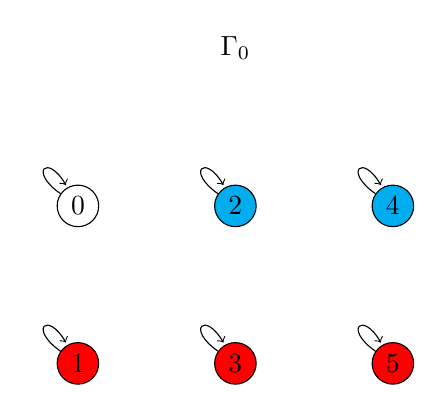
\begin{tikzpicture}[shorten >=1pt,auto,node distance=2cm,
				thin,main node/.style = {circle,draw, inner sep = 0pt, minimum size = 15pt}]
				
				\node[main node,fill=white] (1) {0};
				\node[main node,fill=cyan] [right of = 1](2) {2};
				\node[main node,fill=cyan] [right of = 2](3) {4};
				\node[main node,fill=red] [below of = 1](4) {1};
				\node[main node,fill=red] [right of = 4](5) {3};
				\node[main node,fill=red] [right of = 5](6) {5};
				\node [above of =2] (9) {$\Gamma_0$};
				
				\path (1) edge [in=120,out=145,loop] ();
				\path (2) edge [in=120,out=145,loop] ();
				\path (3) edge [in=120,out=145,loop] ();
				\path (4) edge [in=120,out=145,loop] ();
				\path (5) edge [in=120,out=145,loop] ();
				\path (6) edge [in=120,out=145,loop] ();
				
				\end{tikzpicture}\qquad&\qquad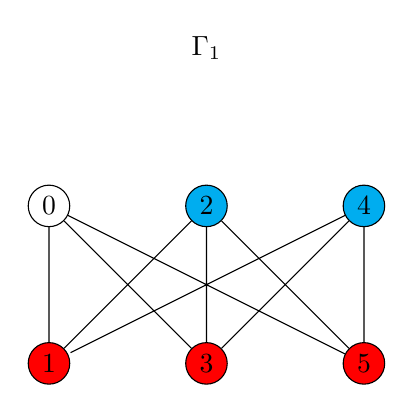
\begin{tikzpicture}[shorten >=1pt,auto,node distance=2cm,
				thin,main node/.style = {circle,draw, inner sep = 0pt, minimum size = 15pt}]
				
				\node[main node,fill=white] (1) {0};
				\node[main node,fill=cyan] [right of = 1](2) {2};
				\node[main node,fill=cyan] [right of = 2](3) {4};
				\node[main node,fill=red] [below of = 1](4) {1};
				\node[main node,fill=red] [right of = 4](5) {3};
				\node[main node,fill=red] [right of = 5](6) {5};
				\node [above of =2] {$\Gamma_1$};
				
				\draw[-] (1)--(4)--(2)--(5)--(3)--(6)--(1)--(5)--(2)--(6)--(3)--(4);
				\end{tikzpicture}\qquad\qquad
				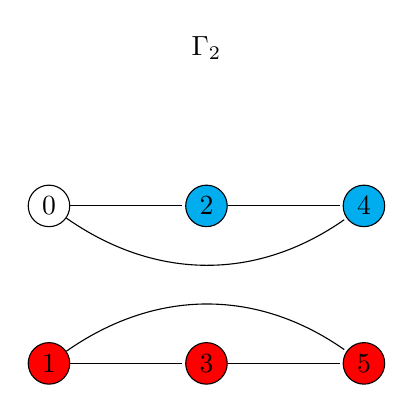
\begin{tikzpicture}[shorten >=1pt,auto,node distance=2cm,
				thin,main node/.style = {circle,draw, inner sep = 0pt, minimum size = 15pt}]	
				\node[main node,fill=white] (1) {0};
				\node[main node,fill=cyan] [right of = 1](2) {2};
				\node[main node,fill=cyan] [right of = 2](3) {4};
				\node[main node,fill=red] [below of = 1](4) {1};
				\node[main node,fill=red] [right of = 4](5) {3};
				\node[main node,fill=red] [right of = 5](6) {5};
				\node [above of =2] {$\Gamma_2$};
				
				\path[-]
				(1)edge node {} (2)
				edge [bend right=35] node {} (3)
				(2)edge node {} (3)
				(4)edge node {} (5)
				edge [bend left=35] node {} (6)
				(5) edge node {} (6);
				\end{tikzpicture}
				\end{aligned}$}\end{center}
		\caption[Graphs of $K_{3,3}$.]{The association scheme of $K_{3,3}$. The subconstituents of vertex $0$ are colored white, red,  and blue respectively.}\label{k33}
	\end{figure}
	The intersection numbers, Krein parameters, and eigenmatrices are
	\[\begin{aligned}L_0 &= \left[\begin{array}{cccc}
	1&0&0\\
	0&1&0\\
	0&0&1\\
	\end{array}\right],\quad L_1 &= \left[\begin{array}{cccc}
	0&3&0\\
	1&0&2\\
	0&3&0\\
	\end{array}\right],\quad L_2 &= \left[\begin{array}{cccc}
	0&0&2\\
	0&2&0\\
	1&0&1\\
	\end{array}\right];\\
	L_0^* &= \left[\begin{array}{cccc}
	1&0&0\\
	0&1&0\\
	0&0&1\\
	\end{array}\right],\quad L_1^* &= \left[\begin{array}{cccc}
	0&4&0\\
	1&2&1\\
	0&4&0\\
	\end{array}\right],\quad L_2^* &= \left[\begin{array}{cccc}
	0&0&1\\
	0&1&0\\
	1&0&0\\
	\end{array}\right];\end{aligned}\]
	\[P = \left[\begin{array}{rrr}
	1&3&2\\
	1&0&-1\\
	1&-3&2\\
	\end{array}\right],\qquad Q = \left[\begin{array}{rrr}
	1&4&1\\
	1&0&-1\\
	1&-2&1\\
	\end{array}\right].\]
	Now consider the $2$-class association scheme determined by the octahedron. The three graphs for this scheme are
	\begin{figure}[H]\begin{center}\scalebox{.7}{$\begin{aligned}
				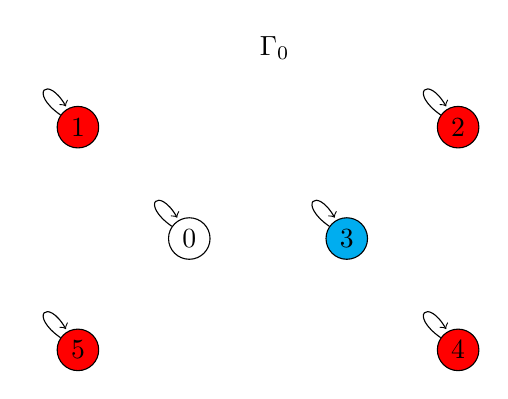
\begin{tikzpicture}[shorten >=1pt,auto,node distance=2cm,
				thin,main node/.style = {circle,draw, inner sep = 0pt, minimum size = 15pt}]
				
				\node[main node,fill=red] (2) {1};
				\node[main node,fill=white] [below right of = 2](1) {0};
				\node[main node,fill=cyan] [right of = 1](6) {3};
				\node[main node,fill=red] [above right of = 6](3) {2};
				\node[main node,fill=red] [below right of = 6](4) {4};
				\node[main node,fill=red] [below left of  = 1](5) {5};
				\node at (2.5,1) (9) {$\Gamma_0$};
				
				\path (1) edge [in=120,out=145,loop] ();
				\path (2) edge [in=120,out=145,loop] ();
				\path (3) edge [in=120,out=145,loop] ();
				\path (4) edge [in=120,out=145,loop] ();
				\path (5) edge [in=120,out=145,loop] ();
				\path (6) edge [in=120,out=145,loop] ();
				
				\end{tikzpicture}\qquad&\qquad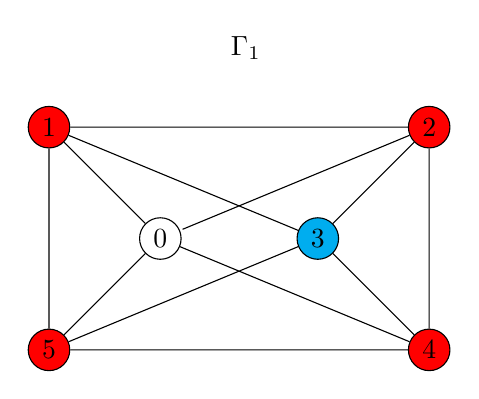
\begin{tikzpicture}[shorten >=1pt,auto,node distance=2cm,
				thin,main node/.style = {circle,draw, inner sep = 0pt, minimum size = 15pt}]
				
				\node[main node,fill=red] (2) {1};
				\node[main node,fill=white] [below right of = 2](1) {0};
				\node[main node,fill=cyan] [right of = 1](6) {3};
				\node[main node,fill=red] [above right of = 6](3) {2};
				\node[main node,fill=red] [below right of = 6](4) {4};
				\node[main node,fill=red] [below left of  = 1](5) {5};
				\node at (2.5,1) (9) {$\Gamma_1$};
				
				\draw[-] (1)--(2)--(3)--(4)--(5)--(2)--(6)--(5)--(1)--(4)--(6)--(3)--(1);
				\end{tikzpicture}\qquad\qquad
				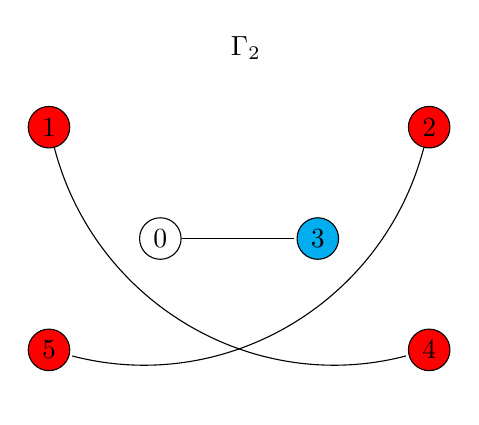
\begin{tikzpicture}[shorten >=1pt,auto,node distance=2cm,
				thin,main node/.style = {circle,draw, inner sep = 0pt, minimum size = 15pt}]	
				
				\node[main node,fill=red] (2) {1};
				\node[main node,fill=white] [below right of = 2](1) {0};
				\node[main node,fill=cyan] [right of = 1](6) {3};
				\node[main node,fill=red] [above right of = 6](3) {2};
				\node[main node,fill=red] [below right of = 6](4) {4};
				\node[main node,fill=red] [below left of  = 1](5) {5};
				\node at (2.5,1) (9) {$\Gamma_2$};
				
				\path[-]
				(1)edge node {} (6)
				(2)edge [bend right=45] node {} (4)
				(3)edge [bend left=45] node {} (5);
				\end{tikzpicture}
				\end{aligned}$}\end{center}
		\caption[Graphs of the octahedron.]{The association scheme of the octahedron. The subconstituents of vertex $0$ are colored white, red, and blue respectively.}\label{octahedron}
	\end{figure}
	The intersection numbers, Krein parameters, and eigenmatrices of this association scheme are
	\[\begin{aligned}
	L_0 &= \left[\begin{array}{cccc}
	1&0&0\\
	0&1&0\\
	0&0&1\\
	\end{array}\right],\quad L_1 &= \left[\begin{array}{cccc}
	0&4&0\\
	1&2&1\\
	0&4&0\\
	\end{array}\right],\quad L_2 &= \left[\begin{array}{cccc}
	0&0&1\\
	0&1&0\\
	1&0&0\\
	\end{array}\right];\\
	L_0^* &= \left[\begin{array}{cccc}
	1&0&0\\
	0&1&0\\
	0&0&1\\
	\end{array}\right],\quad L_1^* &= \left[\begin{array}{cccc}
	0&3&0\\
	1&0&2\\
	0&3&0\\
	\end{array}\right],\quad L_2^* &= \left[\begin{array}{cccc}
	0&0&2\\
	0&2&0\\
	1&0&1\\
	\end{array}\right];
	\end{aligned}\]
	\[P = \left[\begin{array}{rrr}
	1&4&1\\
	1&0&-1\\
	1&-2&1\\
	\end{array}\right],\qquad Q = \left[\begin{array}{rrr}
	1&3&2\\
	1&0&-1\\
	1&-3&2\\
	\end{array}\right].\]
	One may observe that the intersection numbers and the Krein parameters of the two schemes are interchanged, as are the first and second eigenmatrices. This specific example is due to a duality arising from the context of \emph{translation schemes}\index{association schemes!translation schemes}: schemes for which there exists an abelian group $\mathcal{G}$ acting regularly on the vertices with, for each $g\in \mathcal{G}$ and any pair of vertices $x,y\in X$, $(g(x),g(y))\in R_i$ if and only if $(x,y)\in R_i$. When this occurs, we find that $\vert \mathcal{G}\vert = \vert X\vert$ and we may define a dual association scheme $(\hat{X},\hat{\mathcal{R}})$ where $\hat{X} = \left\{\chi:\chi\in \mathcal{G}^*\right\}$ is the group of linear characters of $\mathcal{G}$ and $(\chi,\chi')\in \hat{R}_i$ if and only if $E_i (\chi/\chi') = (\chi/\chi')$ where this division is done entrywise. We further find that our new association scheme is also a translation scheme using the group $\mathcal{G}^*$. In the case of the two association schemes given above, the desired group is $\mathcal{G}\simeq \bbZ_6$ and we find each scheme results as the dual of the other. The pair of schemes listed is a specific case of the more general duality between $\overline{rK_s}$ and $\overline{sK_r}$; that is, the complement of $r$ copies of $K_s$ and the complement of $s$ copies of $K_r$ respectively. In this more general setting, we find that the cyclic group $\bbZ_{rs}$ acts regularly on each set of vertices.
	
	In general, it could be that the automorphism group of a given association scheme is trivial, and thus we do not expect to find a transitive action on the vertices. However we still find interesting properties when we strip away the group requirement and observe at the duality at the level of parameters. We say two association schemes are \emph{formally dual}\index{formal duality} if we may swap the eigenmatrices of one to get the eigenmatrices of the other (equivalently swapping the intersection numbers and Krein parameters of one gives the parameters of the other). In many cases, no dual scheme may exist; consider any association scheme for which the Krein parameters are not integral. However, there are non-trivial examples of formally dual pairs of association schemes, for instance consider the two infinite families generated by de Caen and van Dam \cite{deCaen1999}.  This notion of formal duality still plays a major role in our understanding of the field of association schemes as a whole, motivating many of the questions we will focus on in this thesis. We finish this discussion with one final note: any definition based solely on the parameters of an association scheme gives rise to an analogous definition for the dual. For instance, we find that $K_{3,3}$ is \emph{bipartite}\index{bipartite}, meaning $p^k_{ij}= 0$ whenever $i+j+k\notin2\bbZ$. The dual graph, the octahedron, must then have $q^k_{ij}=0$ whenever $i+j+k\notin2\bbZ$; we will call this \emph{dual-bipartite}\index{bipartite!dual-} or $Q$-bipartite (see \ref{poly}). Similarly, we find that both $K_{3,3}$ and the octahedron are \emph{antipodal graphs}\index{antipodal}: $p^d_{di} = 0$ whenever $i\notin\left\{0,d\right\}$. Both graphs are then what we call \emph{dual-antipodal}\index{antipodal!dual-} or $Q$-antipodal (see \ref{poly}): $q^d_{di}=0$ whenever $i\notin\left\{0,d\right\}$. While there has been much research into bipartite and antipodal graphs, in this thesis we are interested in the implications of these dual properties, seeking when such objects may exist and what combinatorial or geometric structure they impose.
	\section{Feasibility and realizability}
	One main point of interest is whether or not an association scheme exists, given a (possibly partial) parameter set. While existence often cannot be proven without explicitly constructing the scheme, we often may rule out the existence of a scheme due to the values its intersection numbers or Krein parameters must take. In this section we examine three main conditions which we will use throughout this thesis in addition to what we already stated in Lemma \ref{kitchensink}. We begin with an immediate restriction on the intersection numbers:
	\begin{lem}[\cite{Brouwer1989}]\label{intfeas}
		The intersection numbers of an association scheme must be non-negative integers.\qed
	\end{lem}
	This condition is easy to verify since, by definition, each $p^k_{ij}$ is the cardinality of a set. While this property is immediate, it can be a powerful tool to eliminate examples with very little information about the association scheme. Next consider the Krein parameters of our association scheme.
	\begin{lem}[\cite{Scott1973},Krein conditions]\label{kreinfeas}\index{Krein conditions}
		The Krein parameters of an association scheme must be non-negative real numbers.
	\end{lem}
	\begin{proof}
		From equation \eqref{Emult}, we find that $\bigslant{q_{ij}^0}{\vert X\vert},\dots,\bigslant{q_{ij}^d}{\vert X\vert}$ are the eigenvalues of $E_i\circ E_j$. However $E_i\circ E_j\in \BMA$ and therefore it must be symmetric, implying all of its eigenvalues are real. Further, $E_i\circ E_j$ is a principal submatrix of $E_i\otimes E_j$, which has two distinct eigenvalues: $1$ and $0$. Hence $E_i\otimes E_j$ is positive semidefinite and any principal submatrix must share the same property.
	\end{proof}
	The final feasibility condition we will list here is known as the \emph{absolute bound}\index{absolute bound}.
	\begin{lem}[\cite{Neumaier1981},Absolute bound]\label{absolute}
		The multiplicities $m_i$ ($0\leq i\leq d$) of a $d$-class association scheme satisfy:
		\[\sum_{q_{ij}^k\neq 0} m_k\leq\begin{cases}
		m_im_j & \text{ if }i\neq j\\
		\binom{m_i+1}{2} & \text{ if }i= j.
		\end{cases}\]
	\end{lem}
	\begin{proof}
		The sum on the left is the rank of $E_i\circ E_j$, a principal submatrix of the rank $m_im_j$ matrix $E_i\otimes E_j$. Further, if $i=j$, $E_i\circ E_j$ is the entrywise square of $E_i$. Assuming $\text{col}(E_i) = \text{span}(v_1,\dots,v_{m_i})$, the columns of $E_i\circ E_i$ must be linear combinations of the vectors $v_j\circ v_k$ for $1\leq j\leq k\leq d$, a total of $\binom{m_i+1}{2}$ vectors.
	\end{proof}
	There are many other feasibility conditions we may list here including some arising from design theory and others as simple as the handshaking lemma. In this thesis however, we consider the conditions already stated to be a baseline. Thus, we do not claim that any parameter set fulfilling these conditions is guaranteed to correspond to the parameters of some association scheme, rather we instead simply ignore parameter sets which do not fulfill these basic parameter restrictions. We therefore define two separate terms which will be used throughout this thesis, \emph{feasible paramter sets}\index{feasible parameter set} and \emph{realizable parameter sets}\index{realizable parameter set}. 
	\begin{definition}
		A \emph{feasible parameter set} is a set of Krein parameters, intersection numbers, and eigenmatrices such that:
		\begin{itemize}
			\item[FC1:] The Krein parameters satisfy Lemmas \ref{kreinfeas} and \ref{kitchensink} \emph{($\mathit{i'}$) -- ($\mathit{xiii'}$)},
			\item[FC2:] The intersection numbers satisfy Lemmas \ref{intfeas} and \ref{kitchensink} \emph{(i) -- (xiii)},
			\item[FC3:] The integers $m_j = q^0_{jj}$ satisfy Lemma \ref{absolute}.
		\end{itemize}
	\end{definition}
	\begin{definition}
		A feasible parameter set is \emph{realizable} if there exists an association scheme $(X,\cR)$ with the given parameter set.
	\end{definition}
	\section{Imprimitivity}\label{imprimitivity}
	In standard graph theory, one finds many ``products" which take two graphs and build larger graphs out of them. This notion of building larger objects from smaller ones is found in many other fields of mathematics including basic number theory, where fundamental questions arise in identifying which numbers are ``prime". The field of association schemes is no exception; we often distinguish between those schemes whose Bose-Mesner algebra contains smaller non-trivial subalgebras, referring to these as \emph{imprimitive}, and those which contain no non-trivial subalgebras, calling these \emph{primitive}\index{imprimitivity!primitive}. More precisely, an association scheme $(X,\cR)$ is \emph{imprimitive} \index{imprimitivity!imprimitive} if some union of its basis relations is a non-tivial equivalence relation on $X$. Conversely a scheme is \emph{primitive} if no such union of relations exists. Given an imprimitive association scheme, we find two smaller schemes: the \emph{subscheme}\index{imprimitivity!subscheme} and the \emph{quotient scheme}\index{imprimitivity!quotient scheme}; we define both in this section.
	
	We find that a scheme is imprimitive if and only if there exists a disconnected non-trivial relation. For instance, consider the association scheme $K_{3,3}$ depicted in Figure \ref{k33} and note that the union of relations $R_0\cup R_2$ is an equivalence relation with two equivalence classes. Whenever this occurs we call the set of relations which form the equivalence relation a \emph{system of imprimitivity}\index{imprimitivity!systems of -} and denote the set of corresponding indices by $\cI$. In some cases, we may have multiple systems of imprimitivity in our association scheme. For instance consider Example \ref{3cube} and note that $\cI_1 = \left\{0, 2\right\}$ and $\cI_2 = \left\{0, 3\right\}$ are both systems of imprimitivity yet $\cI_1$ has two equivalence classes while $\cI_2$ has four. Thus we must be careful to distinguish between distinct systems of imprimitivity for any given association scheme. In each case, we find that the size of any equivalence class is equal to the sum of the valencies $k_i$ $(i\in\cI)$; hence all classes have the same size for a given system of imprimitivity. In the example of the 3-cube, the size of each equivalence class for $\cI_1$ is $v_0+v_2 = 4$; likewise the size of each equivalence class for $\cI_2$ is $v_0+v_3 = 2$. For all that follows we denote the size of any given equivalence class by $r$ and then the number of equivalence classes by $w$ noting that $\vert X\vert = wr$. For each system of imprimitivity, we define two association schemes which arise: a subscheme and a quotient scheme. We note that the following derivation is non-standard as we will derive the schemes through their Bose-Mesner algebras. We do this to illuminate the duality at play, referring the reader to numerous other sources for a combinatorial derivation (\cite{Brouwer1989},\cite{Rao1984},\cite{Cameron1978},\cite{Martin2007}). 
	
	Suppose $(X,\cR)$ is given with the system of imprimitivity $\cI = \left\{0,i_1,\dots,i_s\right\}$ and equivalence classes $X_1,\dots,X_w$. Then $\left\{A_i\right\}_{i\in\cI}$ forms a basis for a second matrix algebra $\mathbb{B}\subset\BMA$ which is also closed under both matrix and Schur multiplication. We may order the vertices by equivalence classes so that every matrix in $\mathbb{B}$ is block diagonal with $w$ blocks of size $r\times r$. Further, \[\left[\sum_{i\in\cI}A_i\right]_{x,y} = \begin{cases}
	1 \text{ if there exists a }0\leq k\leq w\text{ with }x,y\in X_k,\\
	0 \text{ otherwise.}
	\end{cases}\]
	Thus $\sum_{i\in\cI}A_i = I_w\otimes J_r$ under this vertex ordering. As before, we find that $\mathbb{B}$ is commutative, and thus we may simultaneously diagonalize all matrices in $\mathbb{B}$ giving the basis of idempotents $\left\{E^\prime_i\right\}_{i\in\cI}$. Since our matrices are block diagonal with constant diagonal entries, the dimension of any maximal eigenspace must be a multiple of $w$, the number of blocks on the diagonal. Then, since we have shown the rank $m$ matrix $I_w\otimes J_r\in\mathbb{B}$, we know that $\frac{1}{r}I_w\otimes J_r$ must be one of these matrices as it is has the minimum possible non-zero rank; call it $E^\prime_0$. As these idempotents correspond to the maximal common eigenspaces of $A_0,\dots,A_{i_s}$, every eigenspace of our original Bose-Mesner algebra must be contained in exactly one of these eigenspaces. Thus for $j\in\cI$ define $\hat{j} = \left\{i:E^\prime_j E_i = E_i\right\}$ and we must have $E_j^\prime = \sum_{i\in\hat{j}}E_i$. While $\BMB$ is a vector space closed under both products, it is not a Bose-Mesner algebra as it does not contain the matrix $J$ and thus we cannot fullfill property \emph{(ii)} of our definition. Instead, we find that we may produce a smaller Bose-Mesner algebra by restricting the matrices of our algebra to any of the $r\times r$ blocks on the diagonal, giving $w$ distinct Bose-Mesner algebras on each equivalence class of vertices, noting that $I_r$ and $J_r$ are contained in each smaller algebra. In fact, one may check that the homomorphism $\psi_\ell$ mapping $A_i$ to the $\ell^\text{th}$ $r\times r$ diagonal block of $A_i$ is an algebra isomorphism from $\mathbb{B}$ to a Bose-Mesner algebra on $X_\ell$ preserving both products. The corresponding $s$-class association scheme $\left(X_\ell,\mathcal{R}^\prime\right)$ has relations given by $R_i^\prime = R_i\cap(X_\ell\times X_\ell) = \left.R_i\right\vert_{X_\ell}$ for $i\in\cI$; we call each such association scheme a \emph{subscheme}\index{imprimitivity!subscheme} of $(X,\cR)$. Since matrix multiplication is preserved by our mapping, we find that for $i,j,k\in\cI$, $p^{\prime k}_{ij} = p^k_{ij}$ and thus the intersection numbers match our original scheme for indices within $\cI$. While Schur products are also preserved by $\psi_\ell$, recall that the idempotents of $\mathbb{B}$ were not the same as the idempotents of our original scheme, thus we do not expect our Krein parameters to be preserved. Instead we must determine the parameters $q^{\prime k}_{ij}$ so that 
	\[E_i^\prime\circ E_j^\prime = \frac{1}{\vert X_\ell\vert} \sum_{k\in\cI}q^{\prime k}_{ij}E_k^\prime.\]
	First, note that such constants must exist since $\mathbb{B}$ is closed under entrywise multiplication. Now, recalling that $E_i^\prime = \sum_{a\in\hat{i}} E_a$, we may multiply each side of the above equation by $E_h$ for some $0\leq h\leq d$ and find
	\[\frac{1}{\vert X\vert}\sum_{a\in\hat{i},b\in\hat{j}} q^h_{ab}E_h = \left(E_i^\prime\circ E_j^\prime\right)E_h = \frac{1}{\vert X_\ell\vert}q^{\prime k}_{ij} E_h \]
	where $h\in\hat{k}$. Thus we find
	\begin{equation}q^{\prime k}_{ij} = \frac{1}{w}\sum_{a\in\hat{i},b\in\hat{j}}q^k_{ab}.\end{equation}
	 We note that, while there exist algebra isomorphisms between any pair of subschemes, the $w$ distinct subschemes need not be combinatorially isomorphic; that is, while $\psi_i\circ\psi_j^{-1}$ maps $\BMA_j\rightarrow BMA_i$, there need not be a bijection between $X_j\rightarrow X_i$ for which $(\gamma(x),\gamma(y)\in R_i^\prime$ if and only if $(x,y)\in R_i^\prime$ (see \cite{Jaeger1998} for more discussion on the distinction between ``isomorphic" and "combinatorially isomorphic").
	 	
	We now consider the dual notion, the \emph{quotient scheme}\index{imprimitivity!quotient scheme}, by swapping the roles of our adjacency matrices and idempotents in the above derivation. First observe that Lemma \ref{kitchensink} \emph{($\mathit{i'}$)} applied to any subscheme tells us that $q^{\prime k}_{00} = 0$ for any $k\neq 0$. Thus, our original scheme must have $q^k_{ab} = 0$ whenever $a,b\in\hat{0}$ and $k\notin\hat{0}$. We denote $\cJ = \hat{0}$ and find that this implies the set of matrices $\left\{E_j\right\}_{j\in\cJ}$ is closed under entrywise multiplication. Therefore we have a third commutative matrix algebra $\mathbb{B}^\prime = \text{span}_{j\in\cJ}\left(E_j\right)$ closed under both matrix and Schur multiplication. Since Schur products are always commutative, we may guarantee the existence of Schur idempotents (01-matrices) which span our matrix algebra. Let $\left\{A^\prime_j\right\}_{j\in\cJ}$ correspond to the set of minimal idempotents; that is, the idempotents contained in $\BMB^\prime$ which are not sums of other Schur idempotents in $\BMB^\prime$. These new idempotents correspond to the maximal common Schur-eigenspaces of $\mathbb{B}^\prime$ and, since $\mathbb{B}^\prime\subset\BMA$, we must have sets $\tilde{i} = \left\{j:A^\prime_i\circ A_j = A_j\right\}$ for $i\in\cJ$ giving $A^\prime_i = \sum_{j\in\tilde{i}}A_j$. Further, $\sum_{j\in\cJ} E_j = \frac{1}{r}I_{w}\otimes J_r$ and thus $I_{w}\otimes J_r\in\mathbb{B}^\prime$. This implies one of the these Schur idempotents is $I_w\otimes J_r$; call it $A^\prime_0$, noting that therefore $\tilde{0} = \cI$. Using the set $\left\{E_j\right\}_{j\in \cJ}$ as a basis for $\BMB^\prime$, we find that $A^\prime_iA^\prime_0 = A^\prime_i\left(r\sum_{j\in \cJ} E_j\right) = rA^\prime_i$ and therefore we must have that each $A^\prime_i$ is a block matrix, constant on each block. Thus there exist symmetric matrices $\tilde{A}_i$ for $i\in\cJ$ such that $A^\prime_i = J_r\otimes \tilde{A}_i$ and we may define an algebra homomorphism $\tilde{\psi}$ mapping $A^\prime_i\mapsto \tilde{A}_i$ which preserves entrywise multiplication. We further find that
	\begin{equation}\tilde{\psi}\left(AB\right) = r\tilde{\psi}(A)\tilde{\psi}(B).\label{tildepsiprod}\end{equation}
	Then $\tilde{\psi}(A^\prime_0) = I$, $\tilde{\psi}\left(\sum_{i\in\cJ}A_i\right) =J_w$, and equation \eqref{tildepsiprod} gives us,
	\[\tilde{p}^{\tilde{k}}_{\tilde{i}\tilde{j}} = \frac{1}{r}\sum_{i\in\tilde{i},j\in\tilde{j}}p^k_{ij}\]
	for any choice of $k\in\tilde{k}$; this smaller algebra satisfies all the conditions of a Bose-Mesner algebra. Further, since $\tilde{\psi}$ preserves entrywise products, we find that $\tilde{q}^k_{ij} = q^k_{ij}$ for $i,j,k\in\cJ$. The underlying association scheme of this algebra is called the \emph{quotient scheme}\index{imprimitivity!quotient scheme}. Combinatorially, this is the association scheme $\left(\tilde{X},\tilde{\mathcal{R}}\right)$ where $\tilde{X}$ is the set of $w$ equivalence classes with relations $(X_i,X_j)\in \tilde{R}_{\tilde{i}}$ if there exist $x\in X_i$, $y\in X_j$, and $k\in \tilde{i}$ such that $(x,y)\in R_k$. 
	
	From the above two derivations we find that both the subscheme and the quotient scheme may be obtained by finding a subset of idempotents under one product which are closed under the second product. When this occurs we find a smaller matrix algebra which is isomorphic to a Bose-Mesner algebra on fewer vertices. Thus the only algebraic difference between a subscheme and a dual scheme is simply which set of idempotents we begin with (or rather, with respect to which product we take idempotents for). Throughout this thesis we will use $\tilde{i}$ to describe an index of the quotient scheme and $i^\prime$ an index of the subscheme. Further $\cI$ and $\cJ$ will continue to denote the subset of indices for which
	\[\sum_{i\in\cI} A_i = I_w\otimes J_r = r\sum_{j\in\cJ} E_j.\]
	In summary, we have the following theorem from \cite{Martin2007} as well as a lemma concerning the eigenmatrices of the subscheme and quotient scheme.
	\begin{thm}[\cite{Martin2007}] \label{mmw}The following are equivalent:
		\begin{enumerate}[label=$(\roman*)$]
			\item $(X,\mathbb{R})$ is imprimitive;
%			\item for some $j>0$, $E_j$ has repeated columns;
			\item for some subset $\mathcal{I} = \left\{i_0=0,i_1,\dots,i_s\right\}$ of $\left\{0,1,\dots,d\right\}$ and some ordering of the vertices $\sum_{h=0}^s A_{i_h} = I_w\otimes J_r$ for integers $w$ and $r$ with $\vert X\vert=wr$, $1<w,r<\vert X\vert$;
			\item for some subset $\mathcal{J} = \left\{j_0=0,j_1,\dots,j_s\right\}$ of $\left\{0,1,\dots,d\right\}$ and some ordering of the vertices $\sum_{h=0}^s E_{j_h} = \frac{1}{r}\left(I_w\otimes J_r\right)$ for integers $w$ and $r$ with $\vert X\vert=wr$, $1<w,r<\vert X\vert$.\qed
		\end{enumerate}
	\end{thm}
	\begin{lem}[\cite{Brouwer2003},\cite{Martin2007}]\label{repeatedcols}
	Let $P$ and $Q$ be the first and second eigenmatrix of an imprimitive association scheme with a system of imprimitivity given by $\cI$ and $\cJ$. Let $P^\prime$ be the first eigenmatrix of the subscheme and $\tilde{Q}$ be the second eigenmatrix of the quotient scheme. Then for any $i\in \cI$ and $j\in \cJ$ we have
	\[P^\prime_{\hat{k}i} = P_{ki},\qquad \tilde{Q}_{\tilde{k}j} = Q_{kj}\]
	where $\hat{k}$ is the relation in the subscheme which contains the image of $R_k$ and $\tilde{k}$ is the idempotent of the quotient scheme not orthogonal to the image of $E_k$.\qed
	\end{lem}
	We finish this section by providing an illustration of each type of system of imprimitivity, returning to the example of the $3$-cube. Recall that this association scheme had two systems of imprimitivity: $\cI_1 = \left\{0, 2\right\}$ and $\cI_2 = \left\{0, 3\right\}$. We begin with $\cI_1 = \left\{0,2\right\}$ and display the components of $\Gamma_2$ below.
		\begin{center}\scalebox{.7}{$\begin{aligned}
				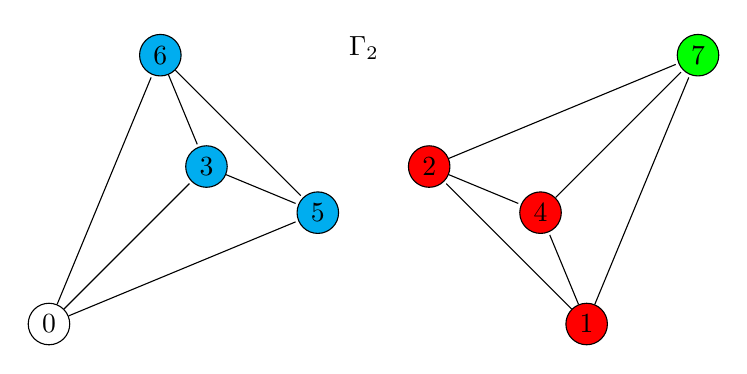
\begin{tikzpicture}[shorten >=1pt,auto,node distance=2cm,
				thin,main node/.style = {circle,draw, inner sep = 0pt, minimum size = 15pt}]
				
				\node[main node,fill=white] (1) {0};
				\node [right of = 1](2) {};
				\node [above of = 1](3) {};
				\node[main node,fill=cyan] [right of = 3](4) {3};
				\node [above right of = 1](5) {};
				\node[main node,fill=cyan] [right of = 5](6) {5};
				\node[main node,fill=cyan] [above of = 5] (7) {6};
				\node [right of = 7](8) {};
				
				\node [below right of =6] (11) {};
				\node[main node,fill=red] [right of = 11](12) {1};
				\node[main node,fill=red] [above of = 11](13) {2};
				\node [right of = 13](14) {};
				\node[main node,fill=red] [above right of = 11](15) {4};
				\node [right of = 15](16) {};
				\node [above of = 15] (17) {};
				\node[main node,fill=green] [right of = 17](18) {7};
				\node at (4,3.5) (9) {$\Gamma_2$};
				
				\path[-]
				(1)edge node {} (4)
				edge node {} (6)
				edge node {} (7)
				(12)edge node {} (13)
				edge node {} (15)
				edge node {} (18)
				(13)edge node {} (15)
				edge node {} (18)
				(4) edge node {} (6)
				(7) edge node {} (4)
				edge node {} (6)
				(15) edge node {} (18);
				\end{tikzpicture}
				\end{aligned}$}\end{center}
			For each of the two components we find a subscheme isomorphic to $K_4$:
		\begin{center}\scalebox{.7}{$\begin{aligned}
				\begin{tikzpicture}[shorten >=1pt,auto,node distance=2cm,
				thin,main node/.style = {circle,draw, inner sep = 0pt, minimum size = 15pt}]
				
				\node[main node,fill=white] (1) {0};
				\node[main node,fill=cyan] [right of = 3](4) {1};
				\node[main node,fill=cyan] [right of = 5](6) {2};
				\node[main node,fill=cyan] [above of = 5] (7) {3};
				\node at (2,4.5) (9) {$\Gamma_0^\prime$};
				
				\path (1) edge [in=120,out=145,loop] ();
				\path (4) edge [in=120,out=145,loop] ();
				\path (6) edge [in=120,out=145,loop] ();
				\path (7) edge [in=120,out=145,loop] ();
				
				\end{tikzpicture}\qquad\qquad
				\begin{tikzpicture}[shorten >=1pt,auto,node distance=2cm,
				thin,main node/.style = {circle,draw, inner sep = 0pt, minimum size = 15pt}]
				
				\node[main node,fill=white] (1) {0};
				\node[main node,fill=cyan] [right of = 3](4) {1};
				\node[main node,fill=cyan] [right of = 5](6) {2};
				\node[main node,fill=cyan] [above of = 5] (7) {3};
				\node at (2,4.5) (9) {$\Gamma_1^\prime$};
				
				\path[-]
				(1)edge node {} (4)
				edge node {} (6)
				edge node {} (7)
				(4) edge node {} (6)
				(7) edge node {} (4)
				edge node {} (6);
				\end{tikzpicture}
				\end{aligned}$}\end{center}
			The quotient scheme is found by collapsing each component to a single point, giving an association scheme isomorphic to $K_2$:
			\begin{center}\scalebox{.7}{$\begin{aligned}
			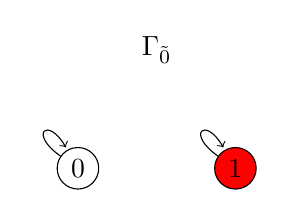
\begin{tikzpicture}[shorten >=1pt,auto,node distance=2cm,
			thin,main node/.style = {circle,draw, inner sep = 0pt, minimum size = 15pt}]
			
			\node[main node,fill=white] (1) {0};
			\node[main node,fill=red] [right of = 1](2) {1};
			\node at (1,1.5) (9) {$\Gamma_{\tilde{0}}$};
			
			\path (1) edge [in=120,out=145,loop] ();
			\path (2) edge [in=120,out=145,loop] ();
			
			\end{tikzpicture}\qquad\qquad
			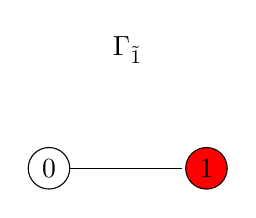
\begin{tikzpicture}[shorten >=1pt,auto,node distance=2cm,
			thin,main node/.style = {circle,draw, inner sep = 0pt, minimum size = 15pt}]
			
			\node[main node,fill=white] (1) {0};
			\node[main node,fill=red] [right of = 1](2) {1};
			\node at (1,1.5) (9) {$\Gamma_{\tilde{1}}$};
			
			\path[-]
			(1)edge node {} (2);
			\end{tikzpicture}
		\end{aligned}$}\end{center}
	Similarly, the system of imprimitivity given by $\cI_2 = \left\{0,3\right\}$ results in the following components of $\Gamma_3$:
	\begin{center}\scalebox{.7}{$\begin{aligned}
			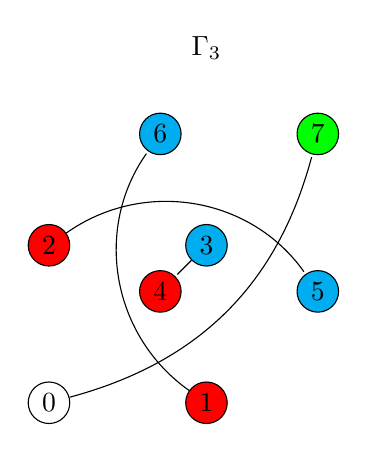
\begin{tikzpicture}[shorten >=1pt,auto,node distance=2cm,
			thin,main node/.style = {circle,draw, inner sep = 0pt, minimum size = 15pt}]
			
			\node[main node,fill=white] (1) {0};
			\node[main node,fill=red] [right of = 1](2) {1};
			\node[main node,fill=red] [above of = 1](3) {2};
			\node[main node,fill=cyan] [right of = 3](4) {3};
			\node[main node,fill=red] [above right of = 1](5) {4};
			\node[main node,fill=cyan] [right of = 5](6) {5};
			\node[main node,fill=cyan] [above of = 5] (7) {6};
			\node[main node,fill=green] [right of = 7](8) {7};
			\node at (2,4.5) (9) {$\Gamma_3$};
			
			\path[-]
			(1) edge [bend right] node {} (8)
			(2) edge [bend left=45] node {} (7)
			(3) edge [bend left=45] node {} (6)
			(4) edge node {} (5);
			\end{tikzpicture}
			\end{aligned}$}\end{center}
		Each component here results in a subscheme isomorphic to $K_2$:
		\begin{center}\scalebox{.7}{$\begin{aligned}
				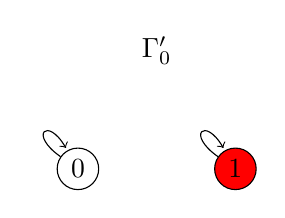
\begin{tikzpicture}[shorten >=1pt,auto,node distance=2cm,
				thin,main node/.style = {circle,draw, inner sep = 0pt, minimum size = 15pt}]
				
				\node[main node,fill=white] (1) {0};
				\node[main node,fill=red] [right of = 1](2) {1};
				\node at (1,1.5) (9) {$\Gamma_0^\prime$};
				
				\path (1) edge [in=120,out=145,loop] ();
				\path (2) edge [in=120,out=145,loop] ();
				
				\end{tikzpicture}\qquad\qquad
				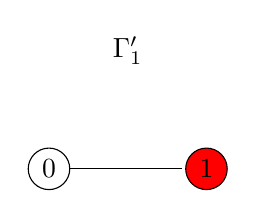
\begin{tikzpicture}[shorten >=1pt,auto,node distance=2cm,
				thin,main node/.style = {circle,draw, inner sep = 0pt, minimum size = 15pt}]
				
				\node[main node,fill=white] (1) {0};
				\node[main node,fill=red] [right of = 1](2) {1};
				\node at (1,1.5) (9) {$\Gamma_1^\prime$};
				
				\path[-]
				(1)edge node {} (2);
				\end{tikzpicture}
				\end{aligned}$}\end{center}
			while, the quotient scheme is isomorphic to $K_4$:
			
			\begin{center}\scalebox{.7}{$\begin{aligned}
					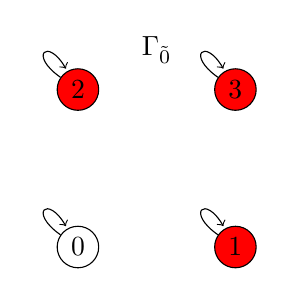
\begin{tikzpicture}[shorten >=1pt,auto,node distance=2cm,
					thin,main node/.style = {circle,draw, inner sep = 0pt, minimum size = 15pt}]
					
					\node[main node,fill=white] (1) {0};
					\node[main node,fill=red] [right of = 1](2) {1};
					\node[main node,fill=red] [above of = 1](3) {2};
					\node[main node,fill=red] [above of =2](4) {3};
					\node at (1,2.5) (9) {$\Gamma_{\tilde{0}}$};
					
					\path (1) edge [in=120,out=145,loop] ();
					\path (2) edge [in=120,out=145,loop] ();
					\path (3) edge [in=120,out=145,loop] ();
					\path (4) edge [in=120,out=145,loop] ();
					
					\end{tikzpicture}\qquad&\qquad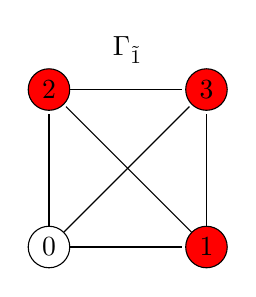
\begin{tikzpicture}[shorten >=1pt,auto,node distance=2cm,
					thin,main node/.style = {circle,draw, inner sep = 0pt, minimum size = 15pt}]
					
					\node[main node,fill=white] (1) {0};
					\node[main node,fill=red] [right of = 1](2) {1};
					\node[main node,fill=red] [above of = 1](3) {2};
					\node[main node,fill=red] [above of =2](4) {3};
					\node at (1,2.5) (9) {$\Gamma_{\tilde{1}}$};
					
					\path[-]
					(1) edge node {} (2)
					edge node {} (3)
					edge node {} (4)
					(2) edge node {} (3)
					edge node {} (4)
					(3) edge node {} (4);
					\end{tikzpicture}
					\end{aligned}$}\end{center}
	It is not typical that the two examples --- both in the same Bose-Mesner algebra --- have subscheme and quotient scheme swapped. This is an artifact of the self-duality of the 3-cube. These schemes correspond to the dual pair of linear codes $\text{rowsp}\left[\begin{array}{ccc}
	1 & 1 & 1
	\end{array}\right]$ and $\text{nullsp}\left[\begin{array}{ccc}
	1 & 1 & 1
	\end{array}\right].$
	\section{Polynomial schemes}\label{poly}
	In this section we define and briefly develop the notion of polynomial association schemes. We again present two dual concepts, $P$-polynomial and $Q$-polynomial, though we will focus primarily on the $Q$-polynomial case outside of this section. Let $(X,\cR)$ be a $d$-class association scheme. We say $(X,\cR)$ is \emph{$Q$-polynomial}\index{$Q$-polynomial}, or \emph{cometric}\index{$Q$-polynomial!cometric}, if there exists an ordering of the idempotents, say $E_0,E_1,\dots,E_d$, such that the Krein parameters satisfy the following conditions:
	\begin{enumerate}
		\item $q^k_{ij} = 0$ whenever $k>i+j$, and
		\item $q^k_{ij} > 0$ whenever $k = i+j$.
	\end{enumerate}
	Additionally, we note that it is sufficient to check only the above conditions with $i=1$ (see \cite[Prop.\ 2.7.1]{Brouwer1989}). Thus we may characterize $Q$-polynomial association schemes as exactly those for which there exists an eigenspace ordering for which the Krein matrix $L_1^*$ is irreducible tridiagonal. Noting that each row of $L_1^*$ sums to $q^0_{11}$, the parameters of $(X,\cR)$ are then entirely determined by its \emph{Krein array}\index{Krein array} $\iota^*(X,\cR) = \left\{b_0^*,\dots,b_{d-1}^*;c_1^*,\dots,c_d^*\right\}$ where $b_i^* = q^i_{1,i+1}$ and $c_i^* = q^{i+1}_{1i}$. When this occurs, we find that $\BMA = \left<E_1\right>_\circ$; that is, $E_1$ generates our entire Bose-Mesner algebra using Schur products. Additionally, for each $0\leq k\leq d$, we may define a single-variable polynomial $q_k(t)$ of degree $k$ so that $Q_{ik} = q_k\left(Q_{i1}\right)$ for $0\leq i\leq d$. This is equivalent to $E_k = \frac{1}{\vert X\vert}q_k\circ\left(\vert X\vert E_1\right)$; that is $q_k$ applied entrywise to $\vert X\vert E_1$ results in $\vert X\vert E_k$ (again see \cite[Prop.\ 2.7.1]{Brouwer1989}). Then we may define one final polynomial $q_{d+1}(t)$ with degree $d+1$ and no repeated roots such that $q_{d+1}\circ(\vert X\vert E_1) = 0$. This immediately implies that $E_1$ has $d+1$ distinct entries and we find it convenient to order the relations according to these values so that $Q_{01}>Q_{11}>\dots>Q_{d1}$; we call this the \emph{natural ordering of relations}\index{natural ordering} with respect to the $Q$-polynomial ordering $E_0,E_1,\dots,E_d$. As is suggested by this definition, it is possible to find multiple $Q$-polynomial orderings for the same association scheme. However, Suzuki \cite{Suzuki1998-2} showed that, with the exception of cycles, any $Q$-polynomial association scheme has at most two $Q$-polynomial orderings. We say a $Q$-polynomial association scheme is \emph{$Q$-bipartite}\index{$Q$-polynomial!$Q$-bipartite} if the Krein parameters satisfy $q^k_{ij} = 0$ whenever $i+j+k\notin 2\bbZ$. We find in this case that $\left\{E_i\right\}_{i\in 2\bbZ}$ serves as a Schur-closed subalgebra. In contrast, we say a $Q$-polynomial scheme is \emph{$Q$-antipodal}\index{$Q$-polynomial!$Q$-antipodal} if $q^k_{dd} = 0$ whenever $k\notin\left\{0,d\right\}$ and thus $\left\{E_0,E_d\right\}$ is a Schur-closed subalgebra. Each case coincides with a system of imprimitivity; the following is Suzuki's theorem concerning these systems.
	\begin{thm}[\cite{Suzuki1998},\cite{Cerzo2009},\cite{Tanaka2011}] \label{suzukiimprim} Suppose $(X,\mathcal{R})$ is an imprimitive cometric association scheme with $Q$-polynomial ordering $E_0,\dots,E_d$ and natural ordering $A_0,\dots,A_d$. Then one of the following holds:
	\begin{enumerate}[label=$(\roman*)$]
		\item $(X,\mathcal{R})$ is $Q$-bipartite and $\mathcal{J} = \left\{0,2,4,\dots\right\}$, $\mathcal{I} = \left\{0,d\right\}$;
		\item $(X,\mathcal{R})$ is $Q$-antipodal and $\mathcal{J} = \left\{0,d\right\}$, $\mathcal{I} = \left\{0,2,4,\dots\right\}$.
	\end{enumerate}
	\end{thm}
	The original theorem in \cite{Suzuki1998} allowed for two exceptional cases, one with $d=4$ and another with $d=6$. These two cases were later ruled out in \cite{Cerzo2009} and \cite{Tanaka2011} respectively.
	
	We now consider the more familiar dual notion: $P$-polynomial association schemes. Again let $(X,\cR)$ be a $d$-class association scheme. We say $(X,\cR)$ is \emph{$P$-polynomial}\index{$P$-polynomial}, or \emph{metric}\index{$P$-polynomial!metric}, if there exists an ordering of the relations, say $A_0,A_1,\dots,A_d$, such that the intersection numbers satisfy the following conditions:
	\begin{enumerate}
		\item $p^k_{ij} = 0$ whenever $k>i+j$, and
		\item $p^k_{ij} > 0$ whenever $k = i+j$.
	\end{enumerate}
	Just as with cometric association schemes, we find that it suffices to check the above conditions only when $i=1$ (\cite[Prop.\ 2.7.1]{Brouwer1989}) and thus an association scheme is $P$-polynomial if and only if there exists an ordering of the relations for which the intersection matrix $(L_1)$ is irreducible tridiagonal. In this case we find that $\BMA= \left<A_1\right>_*$ and it is therefore common to consider a $P$-polynomial scheme synonymous with $\Gamma_1$ --- a \emph{distance-regular graph}; that is $(x,y)\in R_i$ if and only if the distance between $x$ and $y$ in $\Gamma_1$ is $i$. We find analogous results as we saw in the $Q$-polynomial case with \cite[Theorem 4.2.12]{Brouwer1989} and \cite{Taylor1978} giving that any $P$-polynomial association scheme which is not a cycle has at most two $P$-polynomial orderings. Further, we may define \emph{$P$-bipartite}\index{$P$-polynomial!bipartite} (or more commonly \emph{bipartite}) and \emph{$P$-antipodal}\index{$P$-polynomial!antipodal} (\emph{antipodal}) as those schemes for which $p^k_{ij}= 0$ if $i+j+k\not\in 2\bbZ$ and $p^k_{dd}= 0$ whenever $k\not\in\left\{0,d\right\}$ respectively. For these schemes we again find systems of imprimitivity. This time, however, $\mathcal{I} = \left\{0,2,4,\dots\right\}$ and $\mathcal{J} = \left\{0,d\right\}$ correspond to the bipartite scheme while $\mathcal{I} = \left\{0,d\right\}$ and $\mathcal{J} = \left\{0,2,4,\dots\right\}$ for the antipodal scheme. As before, with the exception of cycles, we find that these systems of imprimitivity are all that can occur for $P$-polynomial schemes and note that both can occur within the same association scheme, for example the $3$-cube (more generally the $n$-cube) is both bipartite and antipodal. For details, see Theorem 4.2.1 in the book \cite{Brouwer1989} of Brouwer, et al.\ where credit is given to Smith \cite{Smith1971} and Gardiner \cite{Gardiner1980} where this is reference ``313" in the book \cite{Brouwer1989}.
	
	Despite the close connection between $P$-polynomial and $Q$-polynomial association schemes, we note that many of the theorems mentioned here in the $P$-polynomial case predate their $Q$-polynomial analogues by as much as 30 years. Further, there are many other theorems which are known to be true for metric schemes whose cometric analogues have yet to be proven. For instance Taylor and Levingston showed in 1978 (\cite{Taylor1978}) that the sequence $k_0,k_1,\dots,k_d$ is unimodal, however the $Q$-analogue --- the property that the sequence $m_0,m_1,\dots,m_d$ is unimodal for any $Q$-polynomial ordering --- remains a conjecture to this day. Chapter 6 of \cite{Brouwer1989} details the known examples of distance-regular graphs known at that time --- all tables mentioned here appear in that chapter. Brouwer, et al.\ list 21 classical parameter sets (Tables 6.1 \& 6.2), 15 of which correspond to infinite families, three folded classical graphs (Table 6.3), nine near regular polygons including the generalized polygons (Tables 6.5 \& 6.6), as well as 20 more primitive distance regular graphs (Tables 6.8 \& 6.9). Further they give the known bipartite and antipodal examples (Tables 6.9 \& 6.10 resp.). On the cometric side however, much less is known. Out of the infinite families of $P$-polynomial schemes listed in \cite{Brouwer1989}, five families are also $Q$-polynomial: the Johnson schemes, Hamming schemes, Grassmann schemes, dual polar spaces, and sesquilinear/quadratic forms. More recently \cite{VanDam2005}, Van Dam and Koolen discovered the twisted Grassmann graphs which are also both metric and cometric. The remaining known families $Q$-polynomial association schemes are: linked systems of symmetric designs, mutually unbiased bases, bipartite doubles of some polar spaces, duals of metric translation schemes, two families found by Penttila and Williford \cite{Penttila2011} --- one 4-class $Q$-bipartite and one 3-class primitive --- and one more family found by Moorhouse and Williford \cite{Moorhouse2016}. In addition to these we also know of sporadic examples such as the 22 listed in \cite{Martin2007} and new examples found by King \cite{King2018}. Out of these examples, we note that only the families which are both metric and cometric allow for unbounded $d$. In fact, Bannai and Ito made the following conjecture concerning primitive association schemes.
	\begin{conj*}[Bannai \& Ito] 
		For $d$ sufficiently large, a primitive association scheme with $d$ classes is metric if and only if it is cometric.
	\end{conj*}
	We note that every primitive $2$-class association scheme (connected strongly regular graph) is vacuously both metric and cometric. Thus, in view of the above conjecture, it should not be surprising that the most fruitful place to search for new examples of $Q$-polynomial schemes which are not also metric is the range $3\leq d\leq 6$.